% !TeX spellcheck = en_US
\documentclass[class=article,crop=false]{standalone}
\usepackage{pacco}
\begin{document}
\section{Pitch-shifting via phase vocoder}
We are now ready to focus on our pitch shifting techniques. As we said in the introduction section, we will base our pitch-shifting technique in the well-established approach of the \enf{phase vocoder}.
\subsection{A quick overview of the phase vocoder}
Generally speaking, the term vocoder (from the union of "voice" and "encoder") refers to a class of speech coding that analyzes the information contained in an audio signal (typically speech) and applies them to perform transformations, encryption or compression. The main idea relies in encoding in an envelope signal the tract transmission and vocal excitation separately\footcite[][1]{phasevocoderog}: by means of this separation, the original signal can be discarded while its characteristic features can still be used to modulate other signals or perform operations. The reader may be familiar with the \textit{channel vocoder}, devised by Homer Dudley in 1938\footnote{ibidem} at Bell Labs: this method and its later developments found an important role in voice modification and transformation for technical and artistic purposes, so much that nowadays the channel vocoder is simply known as "vocoder": one can think about the typical "robot voice" in science fiction movies and in the music of electronic artists like Kraftwerk, Herbie Hancock and Giorgio Moroder.\\ The main idea behind this musical effect is using the different informations contained in different bands of frequency of a "carrier signal" to modulate the parameters of a synthesizers, usually the cutoff frequency of a filterbank and the relative impulse responses (the "resonance" of the filters).\par
The phase vocoder was firstly implemented in a paper by Flanagan and Golden\footcite{phasevocoderog}, from Bell Labs. It is indeed a vocoder in the sense that its main functionality consists in taking an input signal, extrapolating its frequency information (amplitude and phase of the different frequency bins), then performing operations on the extrapolated information and lastly using the modified data to synthesize a new signal. The first building block for this procedure (and, really, for any audio processing in time domain) is the \enf{short-time Fourier transform (STFT)}.
\subsection{The short-time Fourier Transform}
The DFT creates a time-fixed frequency representation of a signal as a \textit{periodic} wave: it has no tools to interpret a variation in the frequency information over time. \\In real-life scenarios, we are often interested in analyzing a signal in light of the changes of its frequency content over time. Take into consideration an audio recording with a length of 10 seconds: if we were to feed this sequence of samples into a DFT we would obtain, for each frequency bin (that is, for each $X_n$), one information of magnitude and one information of phase, which would be very noisy and of not much use.\\ We can imagine instead to subdivide our long input signal into shorter "snapshots" taken from a moving frame and then performing a FFT on those windows: this is the core principle behind the STFT.\par
 Since we want to represent the frequency information as accurately as possible, we should consider taking these "snapshots" in such a way that they overlap to each other to a certain degree so that we will be able to interpret the change in frequency information in a smooth way. We could then, frame by frame, perform our desired manipulations and the use a IFFT to go back to time domain and, by overlap-adding our short transformed frames to a buffer, reconstructing an audible signal. The length in samples of each frame is called\footcite[][274]{puckette} \textit{window size}, while the difference between the starting sample of a window and the starting sample of the following window is said \textit{hop size}. Of course, to avoid holes in the STFT, the hop size must be less than the window size.\\
 Another important aspect to take into consideration is \textit{windowing}. As we said, the DFT expects a signal that is periodic. With simple waves like a sine wave this is the case: the wave repeats smoothly since the starting and the ending point are the same.
 \begin{figure}[H]
 	\centering
 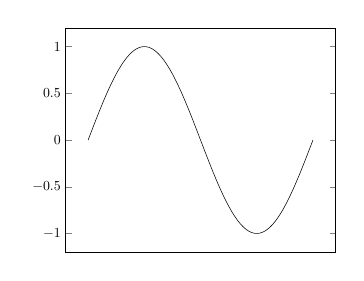
\begin{tikzpicture}[scale=0.5]	
 	\begin{axis}[
 		xtick=\empty
 		]
 		\addplot[samples=300,domain=0:1000] {
 			sin((360*x)/1000)};	
 	\end{axis}
 \end{tikzpicture}
 \end{figure}
 Consider, on the other hand, a wave whose starting and ending points are arbitrary (which is always often the case when dealing with real-world scenarios):
  \begin{figure}[H]
 	\centering
 	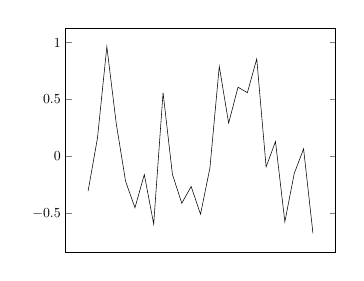
\begin{tikzpicture}[scale=0.5]	
 		\begin{axis}[
 			xtick=\empty
 			]
 			\pgfmathsetseed{1}
 			\addplot[samples=25,domain=0:1000] {
 				(sin((360*x)/1000)+10*rand)/10};	
 		\end{axis}
 	\end{tikzpicture}
 \end{figure}
 This means that the waveform doesn't repeat exactly and there would be a discontinuity (a "jump") in the loop point. This "jump" would be interpreted by the DFT equation as an actual feature of the wave and frequency information would be altered. To face this problem we need a \textit{window function} that not only selects the input in the frame interval, but ensures as well that the signal in the window tapers towards zero at the edge of the window\footcite[][193]{AudioEffects}. There are different type of window functions, each with its own features and drawbacks.\par
 
 Up to now, this whole process can be summarized by the diagram below:
\begin{figure}[H]
	\centering
	\documentclass[crop=false]{standalone}
\usepackage{../pacco}

\begin{document}
	\begin{tikzpicture}[>=stealth']
		
		\draw [fill=red](0,0.5)rectangle ++(12,-0.3) node[pos=0,label=left:$x_n$,anchor=north,yshift=-2 pt] {};
		% Window and Hop Size
		\draw [<->] (1.5,-3) -- (4.5,-3) node [midway,fill=white,above] {\tiny Window Size};
		\draw [<->] (1.5,-2.5) -- (3,-2.5) node [above,midway,fill=white] {\tiny Hop Size};
		\foreach \x in {0,...,4}{
		\draw [top color=red!40,bottom color=white!20](1.5*\x,-0.4-0.55*\x)rectangle ++(3,-0.5) node[midway]{windowed frame};
		}
		\foreach \x in {1.5,3,...,7.5}{
		\draw[dotted] (\x,0.2)--(\x,-3.4);
		}
		\node[circle,below right] at (9.1,-2.6){$\ldots$};
		\begin{scope}[shift={(0,-2)}]
			\foreach \x in {0,...,4}{
			\draw [bottom color=red!60!blue!30,top color=white!20](1.5*\x,-7+0.55*\x)rectangle ++(3,-0.5) node[midway]{windowed frame};
		}
			\draw [fill=red!50!blue!20](0,-8.1)rectangle ++(12,-0.3) node[pos=0,label=left:$X_n$,anchor=north,yshift=-2 pt] {};
		\foreach \x in {1.5,3,...,7.5}{
			\draw[dotted] (\x,-4.6)--(\x,-8.1)node[pos=.96,left]{$+$};
		}
		\node[circle,below right] at (9.1,-4.8){$\ldots$};
	\end{scope}
	\foreach \x in {1.5,3,...,7.5}{
		\draw[->] (\x,-3.4)-- node [pos=1.3]{FFT}(\x,-4.1);
		\draw[->] (\x,-4.45)-- node [draw,rectangle,pos=2.05]{\footnotesize processing}(\x,-4.8);
		\begin{scope}[shift={(0,-0.35)}]
		\draw[->] (\x,-5.15)-- node [pos=1.6]{IFFT}(\x,-5.5);
		\draw[->] (\x,-5.9)--(\x,-6.35);
	\end{scope}
	}
	%%	\draw (0,-0.4)rectangle ++(3,-0.5);
	%	\draw (1.5,-1)rectangle ++(3,-0.5);


	\end{tikzpicture}
\end{document}

\end{figure}
We are now ready for a more formal definition of the STFT\footcite[][221]{dafx}.\\ The short-time Fourier transform of the signal $x_n$ (that from now on we will express as $x(n)$, a function of the sample index $n$) is given by
\begin{equation}\label{stft}
	X(n,k)=\sum_{m=-\infty}^{\infty}x(m)h(n-m)W_N^{mk},\qquad k=0,1,\ldots,N-1
\end{equation}
This formulation is slightly different from Eq. \ref{dft}: while $W_N^{mk}$ has still the meaning of imaginary twiddle factor, now the index of the summation is $m$. This means that at each time index $n$ the signal $x_m$ is weighted by a finite length window $h(n-m)$, with $n-m$ being the window length. This means that the computation of Eq.\ref{stft} can be performed by a finite sum over $m$ with a FFT of length $N$. Typically, $N=n-m$ but it may be desirable to have $N\geqslant n-m$.\\ 
The output $X(n,k)$ is a complex number that expresses the $k$-th (with $0\leqslant k\leqslant N-1$) frequency bin of the frame starting at time $n$. As a complex number, we can refer to Eq.\ref{decomp} to decompose $X(n,k)$:
\begin{equation}\label{decomp2}
	X(n,k)=X_R(n,k)+iX_I(n,k)=|X(n,k)|\cdot e^{i\varphi(n,k)}
\end{equation}
Eq.\ref{decomp2} expresses the result in terms of the \textit{magnitude} $|X(n,k)|$ of the $k$-th frequency bin of the time-varying spectrum and of the \textit{phase} $\varphi(n,k)$ of the same frequency bin. This useful representation will be used later to examine the mechanics of the phase vocoder.\par
Let's now take a deeper look into the window function\footcite[][192]{AudioEffects}. A window function of length $N$ will contain $N$ nonzero samples starting from $n=0$, with a value of 0 at all other samples. There are different window functions, with some examples visible in the figure below. Notice how every window tapers towards 0 at the edges.
\begin{figure}[H]
	\centering
	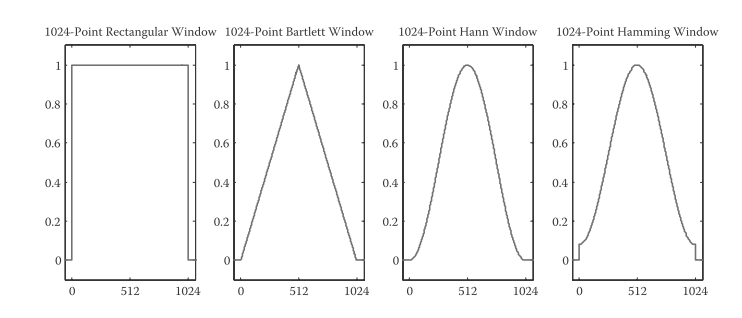
\includegraphics{winfuncs}
	\caption*{Four popular window functions. From \cite{AudioEffects}, p. 192}
	\label{fig:winfuncs}
\end{figure}
Mathematically, the typical window function is defined as follows:
\begin{equation}\label{rect}
	h_{\text{rect}}=\begin{cases}
		1 &0\leqslant n<N\\
		0 &|n|\geqslant N
	\end{cases}
\end{equation}
The window function defined in Eq. \ref{rect} is the \textit{rectangular} window, which is a trivial window that truncates the whole signal at the endpoints. Here there are the definitions of \textit{Bartlett}, \textit{Hann} and \textit{Hamming} windows:
	\begin{align}
		h_{\text{bartlett}}&=\begin{cases}
			1-\left|\frac{2n}{N-1}-1\right| &0\leqslant n<N\\
			0 &|n|\geqslant N
		\end{cases}\\
		h_{\text{hann}}&=\begin{cases}
			\left(1-\cos\left(\frac{2\pi n}{N-1}\right)\right)\cdot\frac{1}{2} &0\leqslant n<N\\
			0 &|n|\geqslant N
		\end{cases}\\
		h_{\text{hamming}}&=\begin{cases}
			0.54-0.46\cos\left(\frac{2\pi n}{N-1}\right) &0\leqslant n<N\\
			0 &|n|\geqslant N
		\end{cases}
	\end{align}
The difference between the different types of windows lies in the ways they handle the phenomenon of \textit{spectral leakage}. Since we are effectively introducing modifications of the original waveform, these modification will create the so-called\footcite[][193]{AudioEffects} \textit{sidelobes} in the frequency domain: artifacts where energy at one frequency bleeds into other frequency bins.
\begin{figure}[H]
	\centering
	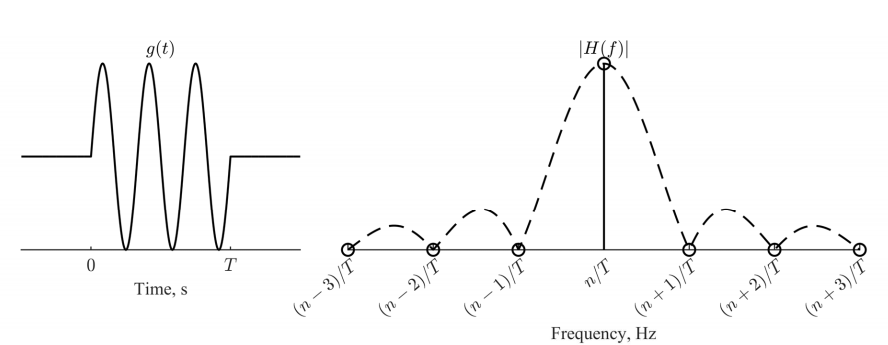
\includegraphics[width=0.8\linewidth]{sidelobez}
	\caption*{Spectral leakage introduced on a sine wave from a rectangular window. The real frequency would be the solid line at $\frac{n}{T}$. From \cite{leakage}, p. 425}
	\label{fig:sidelobez}
\end{figure}
The Bartlett, Hann and Hanning window produce sidelobes with lesser amplitude, but at the cost of reducing the precision with which any given frequency component can be identified. This tradeoff is described as \textit{main lobe width} versus \textit{sidelobe height}.\\Another interesting aspect of the windowing of a signal takes place in the overlap-adding stage of our procedure descripted in the diagram above.
 Since our signal has been windowed, we must take into account how the different windows will overlap once summed together. If the windows do not meet at an amplitude level of 0.5, the sum may exceed 1 with some amplitude modulation between the peaks. A visualization of this situation can be seen in the figure below.  We define the overlap ratio\footcite[][8]{theo} as $1-\frac{\text{hop size}}{\text{window size}}$: valid overlap ratios that preserve amplitude flatness vary from window to window (e.g. for the Hanning window the "safe" overlap ratios are $\frac{1}{2},\frac{2}{3},\frac{3}{4}$).
 % TODO: \usepackage{graphicx} required
 \begin{figure}[H]
 	\centering
 	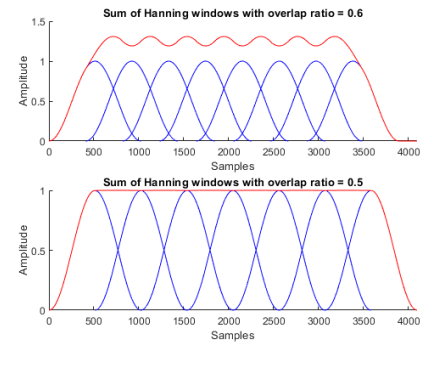
\includegraphics[width=0.8\linewidth]{flatness}
 	\caption*{Various overlap ratios. From \cite{theo}, p. 8}
 	\label{fig:flatness}
 \end{figure}
 \par
To implement the STFT in Python\footnote{This code is based on the Adam Luchies function for STFT (\cite{pystft}). In particular, I did some adjustment to better suite it for audio purpose (i.e. by supporting multichannel audio and by making it compatible with the "librosa" library).} we need to create different functions to perform different vectorial operations. We start by defining a windowing vector with the window coefficients to apply to the signal vector.
\begin{py}
	def windowing(window_function, win_length,num_channels):
	zero_flag = 1 # flag for the while loop
	zeroes = 0
	# call a window function with output points equal to the window length and store it in a vector
	window_vector = window_function(win_length+zeroes)
	
	while zero_flag and (window_vector[0] == 0 or window_vector[-1] == 0): #this excludes the case in which there are zeroes in the middle of the frame but not at the beginning/end but that wouldn't be case with the most common window functions
		start = int(zeroes / 2)
		stop = int(len(window_vector) - start)
		window_vector = window_vector[start : stop] #truncate zeroes at the beginning and the end
		zeroes = len(window_vector) - np.count_nonzero(window_vector) #count zeroes and update
		if zeroes > 0:
			window_vector = window_function(win_length+zeroes) #generate new longer window that hopefully has no zeroes
		else:
			zero_flag = 0
	window_vectors = np.tile(window_vector, (num_channels, 1))
	
	return window_vectors
\end{py}
Note that the windowing function is tweaked to avoid zeroes at the edge of the functions, which would compromise the continuity of the reconstructed signal.\\
We then proceed to create a function that generates our frames from the original signal and stores them as an object of the type \verb*|np.ndarray|, from the library \verb*|numpy|.
\begin{py}
	def generate_frames(x, win_length, hop_length):
	# Input argument checks
	if not isinstance(x, np.ndarray):
		raise ValueError("x is not a numpy array")
	if x.ndim != 2:
		raise ValueError("x must be a 2-dimensional array (channels, samples)")
	if win_length > x.shape[1]:
		raise ValueError("win_length is greater than the number of samples")
	if hop_length <= 0:
		raise ValueError("hop_length must be greater than zero")
	if hop_length > win_length:
		raise ValueError("hop_length cannot be greater than win_length")
	
	# We start by generating start and endpoint for new frames
	startpoint = np.arange(0, x.shape[1] - win_length + 1, hop_length)
	endpoint = startpoint + win_length
	
	# clean possibly too long frames that end after the end of the input
	index = endpoint <= x.shape[1]
	startpoint = startpoint[index]
	endpoint = endpoint[index]
	
	# If the last frame does not include end of the array, we add a frame to include it
	if endpoint[-1] != x.shape[1]:
		endpoint = np.append(endpoint, x.shape[1])
		startpoint = np.append(startpoint, x.shape[1] - win_length)
	
	# we use again list comprehension to create the frames from the original input and stack them
	frames = [x[:, start:stop] for start, stop in zip(startpoint, endpoint)]
	frames = np.stack(frames, axis=-1)
	
	return frames
\end{py}
We then perform the actual STFT on the channels. An issue of the DFT of a fully real input (like a sequence of PCM samples) is the evident "mirroring" of the frequencies around the Nyquist frequency, which corresponds to half the sampling rate and represents the higher frequency with proper representation without any aliasing phenomenon\footcite[][59]{puckette}. This is due to the nature itself of the DFT of a real, which is conjugate symmetric. Consider the $k-th$ bin of the transformed sequence, with $1\leqslant k\leqslant N-1$
$$ X_k =\sum_{n=0}^{N-1}x_ne^{-i\frac{2\pi}{N}kn}$$
And the $(N-k)-th$ bin 

\begin{align*}
	X_{N-k}&=\sum_{n=0}^{N-1}x_ne^{-i\frac{2\pi}{N}(N-k)n}\\
	&=\sum_{n=0}^{N-1}x_ne^{(-i2\pi+i\frac{2\pi}{N}k)n}\\
	&=\sum_{n=0}^{N-1}x_ne^{+i\frac{2\pi}{N}kn}\\
\end{align*}

Consider now the complex conjugate of $X_k$, $(X_k)^*$:

\begin{align*}
	(X_k)^*&=\left(\sum_{n=0}^{N-1}x_ne^{-i\frac{2\pi}{N}kn}\right)^*\\
	&=\sum_{n=0}^{N-1}(x_n)^*e^{+i\frac{2\pi}{N}kn}
\end{align*}

but since $x_n$ is real and therefore has no imaginary part, we have that $(x_n)^*=x_n$ and so

\begin{align*}
	(X_k)^*&=\sum_{n=0}^{N-1}x_ne^{+i\frac{2\pi}{N}kn}\\
	&=X_{N-k}.
\end{align*}

The fact that $X_{N-k}=(X_k)^*$ has the important consequence that the real parts of $X_{N-k}$ and $X_k$ are identical, while their imaginary parts have the same maginitude but opposite signs. An interesting interpretation of this fact lies in the observations that the parts with negative imaginary part (which corresponds to a \textit{negative phase}) are \textit{negative frequencies}, that "spin" in the opposite direction of the positive frequency. 

This fact has, of course, little application in the practice of digital signal processing and this is why the negative frequencies produced by the DFT are usually ditched.  In this implementation, for speed's sake, we used the \verb*|numpy| implementation of real FFT, \verb*|np.fft.rfft|, that manages to cut out from the output the negative aliased frequencies. 
\begin{py}
	def stft(x, n_fft, win_length, hop_length,
	window_function=hann):
	
	# input argument checks
	if type(x) is not np.ndarray:
		raise ValueError("x is not numpy array")
	if win_length > x.shape[1]:
		raise ValueError("win_length is greater than x.shape[1]")
	if hop_length <= 0:
		raise ValueError("hop_length <= 0")
	if hop_length > win_length:
		raise ValueError("hop_length > win_length")
	if n_fft < win_length:
		raise ValueError("n_fft < win_length")
	
	# Number of channels and samples
	channels, samples = x.shape
	
	
	# create an array of window values (as many as the channels of the audio)
	window_vectors = windowing(window_function, win_length,channels)
	
	# overlapping segments
	frames= generate_frames(x,
		win_length, hop_length)
	
	#broadcast windows to all the frames
	frames_windowed = frames * window_vectors[...,np.newaxis]
	# take fft
	stft_res = np.fft.rfft(frames_windowed, n=n_fft, axis=1) #perform the fft from numpy
	
	return stft_res
\end{py}
\subsection{The phase vocoder}
We call the \enf{fundamental frequency} of a sound the lowest frequency component of a waveform, noted $f_0$; we call \enf{harmonics} the components whose frequencies are multiples of the fundamental frequency and we note them as $f_k$. Our ear perceive the fundamental frequency as the pitch of a sound[][8]\footcite{theo} and harmonics as the timbre of a sound. The maxima in the spectral envelope are called \enf{formants}, which characterize the spectral envelope. We perceive the formants as the "fingerprint" of a sound: for example, we can recognize two different people singing a note with the same fundamental frequency because for each fundamental frequency every voice preserves the same formants\footnote{ibidem}.\\ 
Since our perception of pitch is based on a logarithmic scale, we identify pitch relations not as the \textit{difference} between two frequency but as the \textit{ratio} between them. This means that to pitch-shift a sound by a factor $\alpha$ we cannot just add or subtract $\alpha$ from each component of the frequency spectrum (this operation, called \textit{frequency shifting}\footcite[][426]{dafx}, produces a very different and typical effect on the sound) but we must scale the whole spectrum by $\alpha$. This scaling will affect the formants as well, which will compromise the identity of the sound, so we would need to shift them back to their original position.\par
The phase vocoder, as the name suggests, is a method for dealing with all these issues with a \textit{phase} approach. We usually refer to the phase of a sine wave as its principal value in the interval $[-\pi,\pi]$: this is called the \textit{wrapped} phase and, since we desire to perform phase operation, we need to "unwrap" it so that it is a continuous function rather than a modulo $\pi$ function. The figure below\footcite[][242]{dafx} shows the difference between a wrapped phase (solid line) and unwrapped phase (dashed line).
% TODO: \usepackage{graphicx} required
\begin{figure}[H]
	\centering
	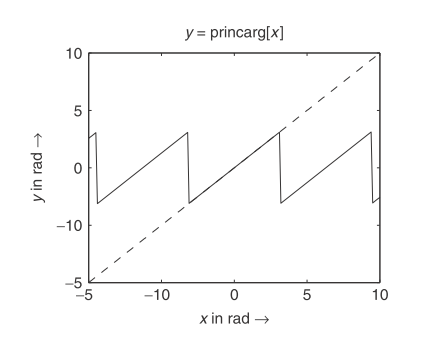
\includegraphics[width=0.65\linewidth]{wrapp}
	\label{fig:wrapp}
\end{figure}
The unwrapped phase is given by
\begin{equation}
	\tilde{\varphi}(n,k)=\frac{2\pi k}{N}+\varphi(n,k)
\end{equation}
We can think of the phase in terms of the "angular speed" of a certain frequency bin around a complex circle (for contrast, we should think of the magnitude as the radius of that complex speed). Higher frequencies "spin" faster and lower frequencies "spin" slower. 
\begin{example}
	Let's use the visualization to consider the phase of a sine wave with frequency 1 Hz. We know that the wave completes a cycle every 1 second, so after 0.5 seconds we expect our phase to be in the following situation:\par
	\begin{minipage}{.4\textwidth}
	\begin{figure}[H]
		\centering
		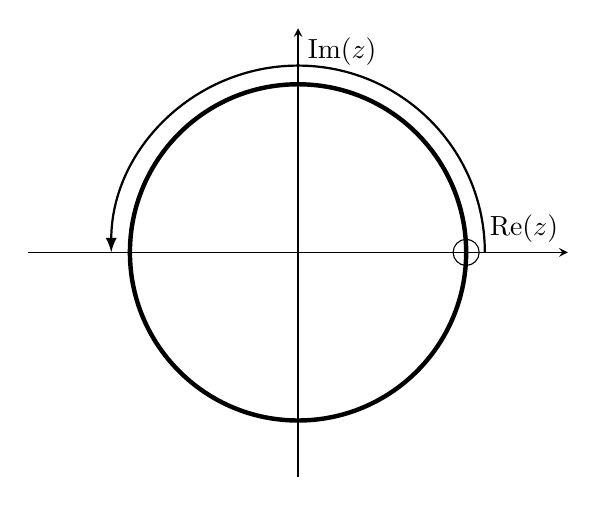
\begin{tikzpicture}
			\begin{axis}[
				xmin=-1.2,
				xmax=1.2,
				ymin=-1.2,
				ymax=1.2,
				axis equal,
				ytick=\empty,
				xtick=\empty,
				axis lines=middle,
				xlabel=Re($z$),
				ylabel=Im($z$),
				disabledatascaling]
				\draw[black,ultra thick] (0,0) circle [radius=0.9];
				\node[circle,draw] at (0.9,0){};
				\draw[-latex,thick] (1,0) arc (0:180:1) node[near start,right] {};
			\end{axis}
		\end{tikzpicture}
	\end{figure}
	\end{minipage}
		\begin{minipage}{.6\textwidth}
		\begin{figure}[H]
			\centering
			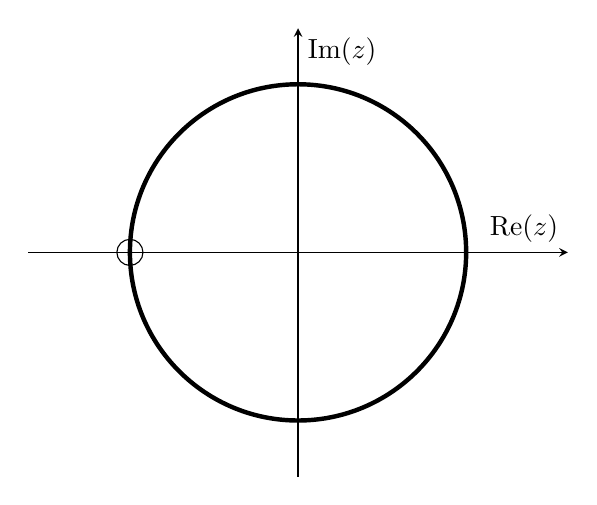
\begin{tikzpicture}
				\begin{axis}[
					xmin=-1.2,
					xmax=1.2,
					ymin=-1.2,
					ymax=1.2,
					axis equal,
					ytick=\empty,
					xtick=\empty,
					axis lines=middle,
					xlabel=Re($z$),
					ylabel=Im($z$),
					disabledatascaling]
					\draw[black,ultra thick] (0,0) circle [radius=0.9];
					\node[circle,draw] at (-0.9,0){};
				\end{axis}
			\end{tikzpicture}
		\end{figure}
	\end{minipage}\\
	Of cours*e, if after 0.5 seconds the phase was in another position around the circle, we wouldn't be dealing with a 1 Hz frequency anymore. The key fact is that \textbf{frequency is uniquely determined by phase}, in particular as the phase derivative with respect to time. This is why we are interested in the unwrapped representation of phase.
\end{example}
So let the starting phase of a measured frequency bin at time $t$ be $\varphi(k,n)$. For a certain frequency bin $f_k$, we expect the phase to "spin" around the circle $f_k\cdot 2\pi h$ times, where $h$ is the hop size (in seconds). This is straightforward: if we take our 1 Hz frequency, after a hop size of 1 second we expect it to have completed a whole rotation. We can then define the expected phase at time t as the expected increment of the phase at the precedent index:
\begin{equation}
	\varphi_t(k,n+1)=\varphi(k,n)+f_k\cdot 2\pi h
\end{equation}
This "target phase\footcite[][198]{AudioEffects}" represents the perfect case of a steady-state sinusoid fitting exactly into a frequency bin with no spectral leakage. Since this would require an infinite-point DFT and since windowing is required, we know that this is not the case. Our real measured phase will have some deviation:
\[
	\varphi_d(k,n+1)=\varphi(k,n)-	\varphi_t(k,n)
\]
This situation is represented in the figure below\footnote{ibidem}:
% TODO: \usepackage{graphicx} required
\begin{figure}[H]
	\centering
	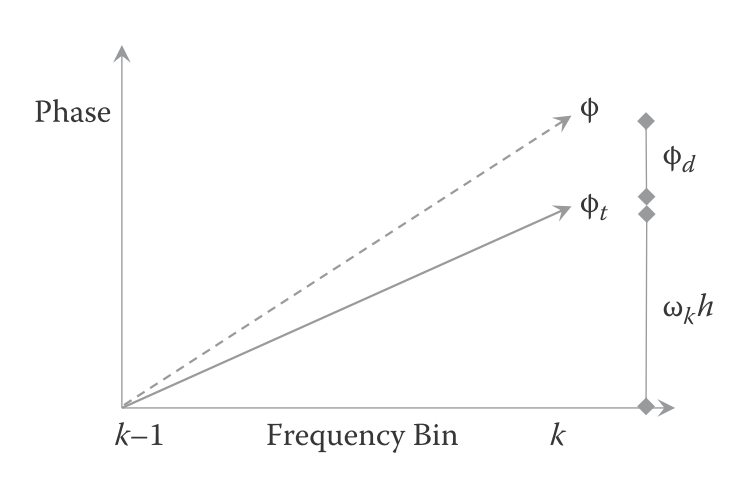
\includegraphics[width=0.6\linewidth]{expphase}
	\label{fig:expphase}
\end{figure}
By comparing the target angle to the real measurement  $\varphi_d(k,n)$, we can know the real unwrapped angle using the corresponding value of this deviation in phase in the range $(-\pi,\pi]$, known as \textit{principal argument}\footcite[][24]{theo}:
\begin{equation}
	\varphi_u(k,n+1)=\varphi_t(k,n)+\text{princarg}(\varphi(k,n+1)-	\varphi_t(k,n+1)).
\end{equation}
where $\text{princarg}(x)=(x+\pi)\mod(2\pi)-\pi$. We can now compute the unwrapped angle difference between measurements $\varphi(k,n)$ and $\varphi(k,n+1)$:
\begin{equation}
	\begin{split}
		\Delta\varphi(k,n+1)&=\varphi_u(k,n+1)-\varphi(k,n)\\
		&=f_k\cdot 2\pi h+\text{princarg}(\varphi(k,n+1)-	\varphi_t(k,n+1))\\
		&=f_k\cdot 2\pi h+\text{princarg}(\varphi(k,n+1)-	\varphi(k,n)-f_k\cdot 2\pi h).
	\end{split}
\end{equation}
As we said in example 2.1, the unwrapped phase difference between 2 consecutive bins contains the information needed to compute the instantaneous frequency for the frequency channel $k$, that can be computed as the phase derivative with respect to time:
\begin{equation}
	\frac{\Delta\varphi(k,n+1)}{2\pi h}
\end{equation}
This operation allows us to have information on how fast phase evolves between 2 consecutive frames.\par
We now have everything we need to perform our spectral operations\footcite[][27]{theo}. Consider $\varphi(k,n)$, the phase of the bin at the $k$-th frequency channel of the $n$-th time frame of the analysis signal. We can compute $\Delta\varphi(k,n+1)$ from $\varphi(k,n)$ and $\varphi(k,n+1)$ and the initialize the phase of the synthesized signal for the first frame as $\varphi_s(k,0)=\varphi(k,0)$. The following synthesis phases are computed as:
\begin{equation}\label{bitchshifting}
	\varphi_s(k,n+1)=\varphi_s(k,n)+\Delta\varphi(k,n+1)\cdot\alpha
\end{equation}
By doing so we preserve the same instantaneous frequency but at the same time we increase (or decrease) the time between the two measurements by a factor of $\alpha$. We are now in control of both the frequency and the time content of each frame. If we approach this flexibility by changing phase relationships and keeping time constant we have effectively devised a \textit{pitch shifting} algorithm, while if we use Eq. \ref{bitchshifting} to change the time while keeping the phase derivative constant we have divesed a \textit{time-stretching} algorithm. \cite{theo} shows the situation in the following plot:
% TODO: \usepackage{graphicx} required
\begin{figure}[H]
	\centering
	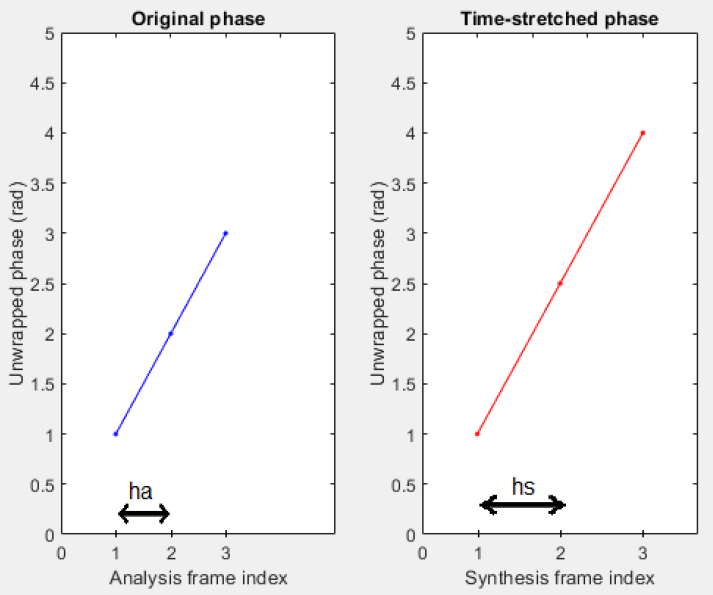
\includegraphics[width=0.6\linewidth]{newphase}
	\label{fig:newphase}
\end{figure}
The phase difference between the 1st and the 2nd synthesis frames is higher, but now the time interval between 2 frames has increased: as a result, the slope of the unwrapped phase remains constant. This mechanism is called \textit{horizontal phase propagation}. \par
After obtaining our modified windows, all we have left to do is performing the ISTFT and overlap-adding our newly modified frames into our new signal.
\subsection{Implementation, limitations and possible improvements}\nocite{jentgent}
We implemented\footnote{inspired from the code for the pitch shifter at \url{https://github.com/JentGent/pitch-shift}} a basic phase-vocoder pitch shifter that uses our previously defined STFT function. One of the problems with implementing phase-vocoder in practice is that the frames of the starting signal and the frames of the synthesized signal may not align, especially when the scaling factor is not a multiple of 2. To solve this problem, we must interpolate (in phase and magnitude) new windows:
\begin{py}
	def interpolate_freq(idxs: np.ndarray, arr):
		start = idxs.astype(int)
		frac = (idxs - start)[None, :, None]
		shifted_arr = np.concatenate((arr[:, 1:, :], np.zeros((arr.shape[0], 1, arr.shape[2]))), axis=1)
		return arr[:, start, :] * (1 - frac) + shifted_arr[:, start, :] * frac
	
	def round_interpolate_freq(idxs: np.ndarray, arr):
		return arr[:, (idxs + 0.5).astype(int), :]
\end{py}
We can now devise a pitch shifting function:
\begin{py}
	def pitch_shifter(\
	audio,scaling,n_fft=4096,win_length=4096,\
	hop_length=1024,window_function=hann,sr=44100):
		stft_data = stft(audio, n_fft, win_length, hop_length, window_function=hann)
		channels, n_stft_frequencies, n_anls_frames = stft_data.shape
		
		#set our scaling factor
		stft_frequencies = np.arange(n_stft_frequencies)
		
		# determine the frequency bins of the new signal. Even if our scaling factor is greater than 1 this doesn't mean that we will be able to represent frequencies beyond the nyquist treshold 
		n_synth_frequencies = int(min(n_stft_frequencies, n_stft_frequencies * scaling))
		synth_frequencies = np.arange(n_synth_frequencies)
		
		# we create the "original" set of frequency bin indices, scaled according to the scaling factor. 
		og_idxs = synth_frequencies / scaling
		
		# calculate the phase difference alignment factor. hop len/win len gives us (in radians after multiplying for 2pi) the change of phase from one frame to the other for sinusoid that makes one cycle over the window lenght. For example, if hop_length=win_length then the pase change is of 2pi, i.e. a full circle. This is needed to "align" the phase changes that are due to the moving window (rather than to frequency changes)
		aligned_phase_diff = np.pi * 2 * hop_length / win_length
		
		#obtain the magnitude and phase vectors from the STFT
		magnitudes = np.abs(stft_data)
		phases = np.angle(stft_data)
		
		#obtain the phase difference array. Concatenate all the phases except the last one in an array along the n_stft_frequencies dimension.
		phase_differences = phases - np.concatenate((np.zeros((channels, n_stft_frequencies, 1)), phases[:, :, :-1]), axis=2)
		
		#We subtract from the phase difference the phase variation that is due to the hopping window. This will prevent spectral leakage caused by the algorithm misinterpreting the phase progression as variation in frequency (and consequently introducing artifacts).
		phase_differences -= (stft_frequencies * aligned_phase_diff)[None, :, None]
		
		#wrap around 2pi
		phase_differences = np.mod(phase_differences + np.pi, np.pi * 2) - np.pi
		
		#interpolation procedures
		
		#we need to create the new framework to "fit" our shifted windows.
		shifted_magnitudes = interpolate_freq(og_idxs, magnitudes)
		shifted_phase_differences = interpolate_freq(og_idxs, phase_differences) * scaling
		
		#again, adjust the phase differences removing the natural variation of phase given by the hopping window.
		shifted_phase_differences += (synth_frequencies * aligned_phase_diff)[None, :, None]
		
		#cumulatively sum all the phase differences to obtain the new phase values!
		shifted_phases = np.cumsum(shifted_phase_differences, axis=2)
		
		#create the synthesis signal by combining the magnitudes with their phases in a complex numbers
		synth_stft = shifted_magnitudes * np.exp(shifted_phases * 1j)
		#fill with zeroes any possible "holes" given by discarded frequnecies
		synth_stft = np.concatenate((synth_stft, np.zeros((channels, n_stft_frequencies - n_synth_frequencies, n_anls_frames))), axis=1)
		
		#perform the inverse fourier transform and display the pitch shifted audio
		new_audio = librosa.istft(synth_stft, hop_length=hop_length, win_length=win_length, n_fft=n_fft)
		idisplay.display(idisplay.Audio(new_audio,rate=sr))
\end{py}
Notice how the key passage of the shifting for the factor $\alpha$ is in line 37 and is the translation of Eq. \ref{bitchshifting}.
This naive implementation of pitch shifting presents various audio artifacts such as:
\begin{itemize}
	\item chorus effect: the sensation that the sound comes from many, slightly detuned, sources;
	\item transient smearing: the transients (high-energy impacts of short duration in the waveform) appear dispersed in time, with some pre-ringing effect and some reverberation;
	\item phasiness: the sound is thinned and harmonically confused (similarly to a guitar effected with a "phaser" pedal);
	\item beatings: the individual harmonics appear like their amplitude is being modulated by a sine wave of varying frequency.
\end{itemize}
These artifacts are due to the loss of vertical coherence in the phase vocoder\footcite[][3]{Laroche}. We preserved phase coherence "horizontally' (that is, along the time/frame axis) but we did nothing to preserve the phase consistency \textit{across} the different frequency bins. Since a pure sinusoid in time domain is actually spread over several frequency bins in frequency domain due to sidelobes and spectral leakage, the phase vocoder processes each of these frequency bins individually. This means that what was originally a sine wave with frequency $f$ is now interpreted as a sum of sine waves with frequencies $f\pm \frac{1}{N-1},\frac{1}{N-2},\ldots$ with decaying amplitude as we depart from the original value of $f$. This explains the chorus effect and the phasiness.\par
A solution of this issue has been proposed by \cite{Laroche} in what is called a \textit{phase-locked vocoder}: here phase values of the frequency channels which correspond to the same component are changed together on the basis of grouping made with peak detection on the magnitude spectrum. Frequency bins are then assigned to their closest peak and only one instantaneous frequency, which is inherited by all the frequency bins in one group, is computer for each peak. In \cite{fuckhorizontalcoherence}, for example, the phasiness is further reduced by not completely preserving horizontal coherence and slightly translating frames in time.\par
Another interesting extension of the phase vocoder is the so-called "phase vocoder done right", in \cite{doneright}: this approach introduces, beside the classical horizontal propagation, the concept of \textit{vertical} propagation: this means that the algorithm is not only modifying phase information in the time domain, but also in the \textit{frequency} domain. Depending on the magnitude of the different bins, the "phase vocoder done right" chooses for each step whether to propagate phase in the time or in the frequency direction. This algorithm uses a max heap\footcite[][3]{doneright} data structure (where elements can be pushed into a max heap and the element popped is always the maximum value of the heap). The main idea behind the algorithm is storing in a max heap elements of the type $(G_h,k_h,n_h)$ where $G_h$ is the magnitude of the bin, $k_h$ is its frequency index and $n_h$ is its time index. Every iteration, we pop the element with maximum magnitude from the heap and we look at the element in the same frequency bin but at the next time index $(G'_h,k_h,n_h+1)$. If $G'_h$ is above a certain threshold, then we propagate phase in the time direction by computing the synthesis phase and adding the new element to the heap; otherwise if $G'_h$ is below the threshold we assign to this bin a random phase value and we pass to the next element of the heap. At this point, the next element of the heap can belong to the $n_h$ group of frames or to the $n_h+1$ group of frames that we have just computed. In the first case we repeat the procedure already described; otherwise we look at the elements $(G''_h,k_h+1,n_h+1)$ and $(G''_h,k_h-1,n_h+1)$, which are the elements vertically adjacent to the element in time frame $n_h+1$ that we have just calculated. The process is the repeated until all synthesis bins have been visited.
% TODO: \usepackage{graphicx} required
\begin{figure}[h]
	\centering
	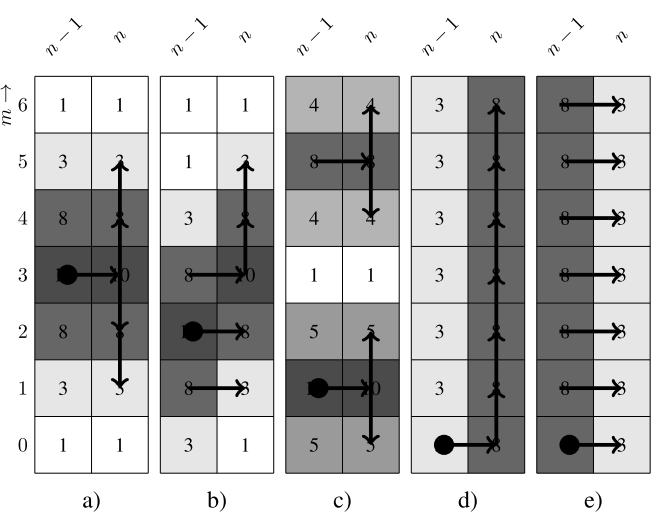
\includegraphics[width=0.7\linewidth]{phasevocoderdoneright}
	\caption*{Diagram of the "phase vocoder done right". From \cite{doneright}, p. 4}
	\label{fig:phasevocoderdoneright}
\end{figure}
\end{document}